\documentclass[12pt]{article}
\usepackage{fancyhdr}
\usepackage{amsmath,amsfonts,enumerate}
\usepackage{color,graphicx}
\usepackage{tikz}
\usepackage{pgfplots}
\usetikzlibrary{arrows,positioning,shapes,calc,matrix}
\pagestyle{fancy}
%%%%%%%%%%%%%%%%%%%%%%%%%%%%%%%%%%%%%%%%%%%%%%%%%
% Course customization
%%%%%%%%%%%%%%%%%%%%%%%%%%%%%%%%%%%%%%%%%%%%%%%%%
\newcommand{\masunitnumber}{CENG 403}
\newcommand{\examdate}{January 2025}
\newcommand{\academicyear}{2024-2025}
\newcommand{\semester}{I}
\newcommand{\coursename}{Deep Learning - Self-Attention and Transformers}
\newcommand{\numberofhours}{3}
%%%%%%%%%%%%%%%%%%%%%%%%%%%%%%%%%%%%%%%%%%%%%%%%%
% CUSTOM SPACING COMMANDS FOR ANSWER SPACES
%%%%%%%%%%%%%%%%%%%%%%%%%%%%%%%%%%%%%%%%%%%%%%%%%
% Flexible answer space command - you can adjust the size
\newcommand{\answerspace}[1]{\vspace{#1}}
% Standard spacing commands with predefined sizes
\newcommand{\questionspace}{\vspace{3cm}}        % Space between questions
\newcommand{\subquestionspace}{\vspace{2.5cm}}   % Standard space for sub-questions
\newcommand{\shortanswer}{\vspace{2cm}}          % For simple calculations
\newcommand{\mediumanswer}{\vspace{3cm}}         % For moderate complexity
\newcommand{\longanswer}{\vspace{4cm}}           % For complex problems
\newcommand{\journalspace}{\vspace{4.5cm}}       % For detailed explanations
%%%%%%%%%%%%%%%%%%%%%%%%%%%%%%%%%%%%%%%%%%%%%%%%%
% Don't touch anything from here till instructions
% to candidates
%%%%%%%%%%%%%%%%%%%%%%%%%%%%%%%%%%%%%%%%%%%%%%%%%
\lhead{}
\rhead{}
\chead{{\bf MIDDLE EAST TECHNICAL UNIVERSITY}}
\lfoot{}
\rfoot{}
\cfoot{}
\begin{document}
\setlength{\headsep}{5truemm}
\setlength{\headheight}{14.5truemm}
\setlength{\voffset}{-0.45truein}
\renewcommand{\headrulewidth}{0.0pt}
\begin{center}
SEMESTER \semester\ EXAMINATION \academicyear
\end{center}
\begin{center}
{\bf \masunitnumber\ -- \coursename}
\end{center}
\vspace{20truemm}
\noindent \examdate\hspace{45truemm} TIME ALLOWED: \numberofhours\ HOURS
\vspace{19truemm}
\hrule
\vspace{19truemm}
\noindent\underline{INSTRUCTIONS TO CANDIDATES}
\vspace{8truemm}
%%%%%%%%%%%%%%%%%%%%%%%%%%%%%%%%%%%%%%%%%%%%%%%%%%%%%%
% Exam instructions
%%%%%%%%%%%%%%%%%%%%%%%%%%%%%%%%%%%%%%%%%%%%%%%%%%%%%%
\begin{enumerate}
\item This examination paper contains {\bf SIX (6)} questions and comprises 
{\bf EIGHT (8)} printed pages.
\item Answer all questions. 
The marks for each question are indicated at the beginning of each question.
\item Answer each question beginning on a {\bf FRESH} page of the answer book.
\item This {\bf IS NOT an OPEN BOOK} exam.
\item Calculators are allowed for numerical computations.
\item Show all mathematical derivations and computational steps clearly.
\item For matrix operations, clearly indicate dimensions and show intermediate steps.
\item Draw clear diagrams where requested and label all components.
\end{enumerate}
%%%%%%%%%%%%%%%%%%%%%%%%%%%%%%%%%%%%%%%%%%%%%%%%%
% leave this as it is
%%%%%%%%%%%%%%%%%%%%%%%%%%%%%%%%%%%%%%%%%%%%%%%%%
\newpage
\lhead{}
\rhead{\masunitnumber}
\chead{}
\lfoot{}
\cfoot{\thepage}
\rfoot{}
\setlength{\footskip}{45pt}
%%%%%%%%%%%%%%%%%%%%%%%%%%%%%%%%%%%%%%%%%%%%%%%%%%
% EXAM QUESTIONS WITH ANSWER SPACES
%%%%%%%%%%%%%%%%%%%%%%%%%%%%%%%%%%%%%%%%%%%%%%%%%%
\paragraph{Question 1. Text Encoding Methods and Challenges}\hfill (20 marks)\\
Deep learning models can process text using different encoding approaches, each with distinct advantages and limitations.

\begin{enumerate}[(a)]
    \item Compare and contrast three text encoding methods: character-level encoding, word-level encoding (word embeddings), and subword-level encoding (Byte Pair Encoding). For each method, discuss: \hfill (12 marks)
    \begin{itemize}
        \item How new/unseen words are handled
        \item Vocabulary size considerations
        \item Suitability for morphologically rich languages (e.g., Turkish)
    \end{itemize}
    
    \journalspace
    
    \item Explain why Byte Pair Encoding might be particularly advantageous for machine translation between languages that share some common subword structures. Provide a concrete example. \hfill (8 marks)
    
    \mediumanswer
\end{enumerate}

\newpage
\paragraph{Question 2. RNN-based Sequence-to-Sequence Models}\hfill (25 marks)\\
Consider the encoder-decoder architecture used for neural machine translation in 2014, which achieved state-of-the-art results but had significant limitations.

\begin{enumerate}[(a)]
    \item Complete the diagram below by adding the missing components of the encoder-decoder architecture for machine translation. Add labels for: encoder RNN cells, decoder RNN cells, hidden states ($h_1, h_2, h_3, h_4$), input embeddings, output predictions, and the bottleneck representation. \hfill (8 marks)
    
    \begin{center}
    \begin{tikzpicture}[scale=0.8, every node/.style={scale=0.8}]
        % Input sequence
        \node at (0,0) {$x_1$};
        \node at (1.5,0) {$x_2$};
        \node at (3,0) {$x_3$};
        \node at (4.5,0) {$<$EOS$>$};
        
        % Encoder cells (students need to add)
        \draw[dashed] (0,1) rectangle (1,2);
        \draw[dashed] (1.5,1) rectangle (2.5,2);
        \draw[dashed] (3,1) rectangle (4,2);
        \draw[dashed] (4.5,1) rectangle (5.5,2);
        
        % Arrow to decoder
        \draw[thick,->] (5.5,1.5) -- (7,1.5);
        
        % Decoder cells (students need to add)
        \draw[dashed] (7.5,1) rectangle (8.5,2);
        \draw[dashed] (9,1) rectangle (10,2);
        \draw[dashed] (10.5,1) rectangle (11.5,2);
        
        % Output sequence
        \node at (8,2.5) {$y_1$};
        \node at (9.5,2.5) {$y_2$};
        \node at (11,2.5) {$y_3$};
        
        % Labels for students to complete
        \node[above] at (2.25,2.2) {\textit{Encoder}};
        \node[above] at (9.5,2.8) {\textit{Decoder}};
        \node at (6.25,1) {\textit{?}};
    \end{tikzpicture}
    \end{center}
    
    \shortanswer
    
    \item Explain the long-term dependency problem in this architecture. Why does this problem become severe when translating long sentences (e.g., 100+ words)? Discuss both forward pass and backward pass challenges. \hfill (10 marks)
    
    \longanswer
    
    \item Calculate the effective depth of the unfolded network when translating a 50-word source sentence to a 50-word target sentence. Explain why this creates optimization difficulties. \hfill (7 marks)
    
    \mediumanswer
\end{enumerate}

\newpage
\paragraph{Question 3. Attention Mechanism and Bahdanau Attention}\hfill (30 marks)\\
The attention mechanism was introduced to address the limitations of basic encoder-decoder models.

\begin{enumerate}[(a)]
    \item Explain the core intuition behind attention mechanism. How does it solve the long-term dependency problem in encoder-decoder models? \hfill (8 marks)
    
    \mediumanswer
    
    \item Given decoder hidden state $h_i^{dec}$ and encoder hidden states $h_1^{enc}, h_2^{enc}, \ldots, h_T^{enc}$, write the mathematical formulation for Bahdanau attention mechanism. Include: \hfill (12 marks)
    \begin{itemize}
        \item Alignment score calculation using a 2-layer MLP
        \item Attention weight normalization
        \item Context vector computation
    \end{itemize}
    
    \journalspace
    
    \item Compare Bahdanau attention with three alternative similarity measures: cosine similarity, scaled dot product, and simple dot product. Write the mathematical expressions and discuss the computational complexity of each. \hfill (10 marks)
    
    \longanswer
\end{enumerate}

\newpage
\paragraph{Question 4. Self-Attention Mechanism and Scaled Dot-Product Attention}\hfill (35 marks)\\
Self-attention allows parallel processing of sequence elements and forms the foundation of transformer architectures.

\begin{enumerate}[(a)]
    \item Starting from the basic self-attention concept, derive the complete mathematical formulation for scaled dot-product attention. Given input embeddings $E_0, E_1, \ldots, E_{T-1}$, show how to compute: \hfill (15 marks)
    \begin{itemize}
        \item Query, Key, and Value matrices using learnable parameters $W_Q$, $W_K$, $W_V$
        \item Attention scores and their normalization
        \item Final output computation
    \end{itemize}
    Include the scaling factor and explain its necessity.
    
    \journalspace
    
    \item Consider two word embeddings $x_1 = [1, 2, 0]$ and $x_2 = [0, 1, 2]$ with dimension $d=3$. Given: \hfill (12 marks)
    $$W_Q = \begin{bmatrix} 1 & 0 & 1 \\ 0 & 1 & 0 \\ 1 & 1 & 0 \end{bmatrix}, \quad W_K = \begin{bmatrix} 0 & 1 & 0 \\ 1 & 0 & 1 \\ 0 & 0 & 1 \end{bmatrix}, \quad W_V = \begin{bmatrix} 1 & 1 & 0 \\ 0 & 1 & 1 \\ 1 & 0 & 1 \end{bmatrix}$$
    
    Calculate the updated representation for $x_1$ using scaled dot-product attention. Show all intermediate steps including query/key/value computation, attention scores, and final weighted combination.
    
    \journalspace
    
    \item Explain why self-attention is position-invariant and why this is both an advantage and a limitation. How does this property affect the computational complexity compared to RNNs? \hfill (8 marks)
    
    \mediumanswer
\end{enumerate}

\newpage
\paragraph{Question 5. Transformer Architecture and Multi-Head Attention}\hfill (40 marks)\\
The transformer architecture revolutionized sequence modeling by replacing recurrence with attention mechanisms.

\begin{enumerate}[(a)]
    \item Complete the transformer encoder block diagram below by filling in the missing components and connections. Add: multi-head self-attention layers, skip connections, layer normalization blocks, and feed-forward network. Use arrows to show information flow and label each component. \hfill (12 marks)
    
    \begin{center}
    \begin{tikzpicture}[scale=0.8, node distance=1.5cm]
        % Input embeddings
        \node[draw, rectangle, minimum width=3cm] (input) at (0,0) {Input Embeddings + Positional Encoding};
        
        % Placeholder for multi-head attention (students complete)
        \draw[dashed] (-1,2) rectangle (1,3);
        \node at (0,2.5) {?};
        
        % Placeholder for add & norm
        \draw[dashed] (-1,4) rectangle (1,5);
        \node at (0,4.5) {?};
        
        % Placeholder for feed forward
        \draw[dashed] (-1,6) rectangle (1,7);
        \node at (0,6.5) {?};
        
        % Placeholder for add & norm
        \draw[dashed] (-1,8) rectangle (1,9);
        \node at (0,8.5) {?};
        
        % Output
        \node[draw, rectangle, minimum width=3cm] (output) at (0,10) {Output Representations};
        
        % Students need to add arrows and skip connections
        \node[right] at (1.5,5) {\textbf{Add missing components and connections}};
        
    \end{tikzpicture}
    \end{center}
    
    \shortanswer
    
    \item Explain multi-head attention mechanism. Why do we use multiple attention heads instead of a single large attention mechanism? Include the mathematical formulation showing how heads are computed in parallel and combined. \hfill (10 marks)
    
    \longanswer
    
    \item Design and explain a positional encoding scheme. Compare learnable positional embeddings vs. trigonometric positional encoding. What are the trade-offs, especially regarding generalization to longer sequences than seen during training? \hfill (10 marks)
    
    \longanswer
    
    \item A transformer decoder differs from the encoder in two key ways. Explain: \hfill (8 marks)
    \begin{itemize}
        \item Masked self-attention and why it's necessary
        \item Cross-attention mechanism and how it connects to the encoder
    \end{itemize}
    
    \mediumanswer
\end{enumerate}

\newpage
\paragraph{Question 6. Attention Visualization and Interpretation}\hfill (20 marks)\\
Understanding attention patterns helps interpret how transformers process language and resolve ambiguities.

\begin{enumerate}[(a)]
    \item Below is a partial attention heatmap for the sentence "The animal didn't cross the street because it was too tired." The attention weights show how much each word attends to every other word. Complete the missing attention patterns and explain what linguistic phenomenon this demonstrates. \hfill (10 marks)
    
    \begin{center}
    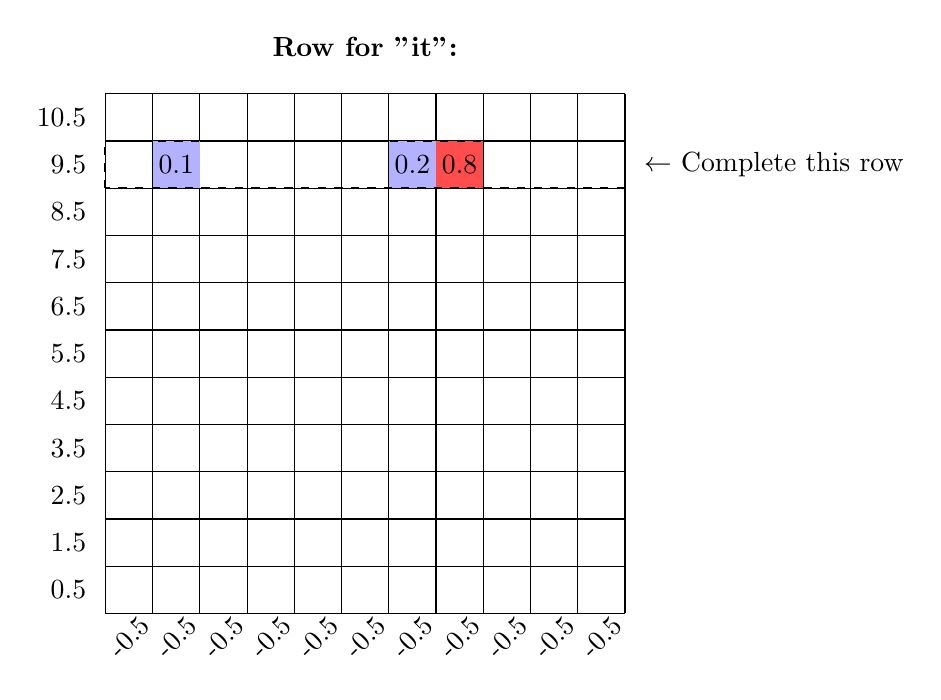
\begin{tikzpicture}[scale=0.6]
        % Define words
        \def\words{{"The", "animal", "didn't", "cross", "the", "street", "because", "it", "was", "too", "tired"}}
        \def\n{11}
        
        % Draw word labels on x-axis
        \foreach \i in {0,...,10} {
            \pgfmathparse{\words[\i]}
            \node[rotate=45] at (\i+0.5, -0.5) {\pgfmathresult};
        }
        
        % Draw word labels on y-axis  
        \foreach \i in {0,...,10} {
            \pgfmathparse{\words[\i]}
            \node[anchor=east] at (-0.2, 10.5-\i) {\pgfmathresult};
        }
        
        % Draw grid
        \draw[step=1] (0,0) grid (11,11);
        
        % High attention for "it" to "animal" (students should complete this)
        \fill[red!70] (7,9) rectangle (8,10);
        \node at (7.5,9.5) {0.8};
        
        % Some given attention weights
        \fill[blue!30] (1,9) rectangle (2,10);
        \node at (1.5,9.5) {0.1};
        
        \fill[blue!30] (6,9) rectangle (7,10);
        \node at (6.5,9.5) {0.2};
        
        % Students need to fill in more patterns
        \node at (5.5, 12) {\textbf{Row for "it": }};
        
        % Mark areas for students to complete
        \draw[dashed, thick] (0,9) rectangle (11,10);
        \node[right] at (11.2, 9.5) {$\leftarrow$ Complete this row};
        
    \end{tikzpicture}
    \end{center}
    
    \mediumanswer
    
    \item Draw a transformer encoder block processing the sequence ["thinking", "machines", "learn"]. Show: \hfill (10 marks)
    \begin{itemize}
        \item Input embeddings with positional encoding addition
        \item Query, Key, Value projections 
        \item Attention score computation between "thinking" and all words
        \item Skip connections and layer normalization
    \end{itemize}
    
    \begin{center}
    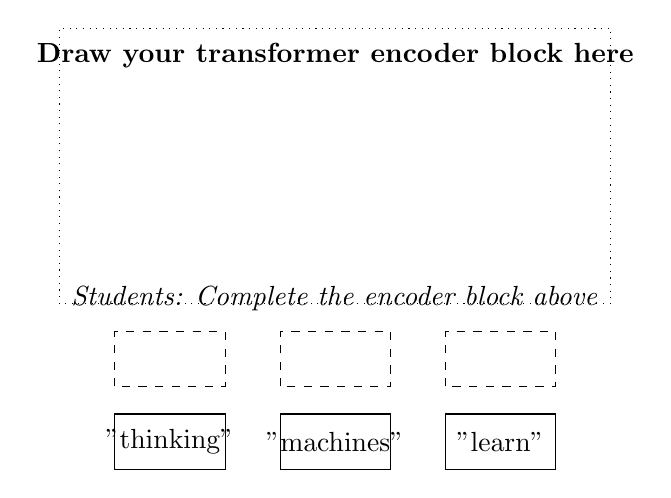
\begin{tikzpicture}[scale=0.7]
        % Input embeddings
        \draw (0,0) rectangle (2,1);
        \node at (1,0.5) {"thinking"};
        
        \draw (3,0) rectangle (5,1);
        \node at (4,0.5) {"machines"};
        
        \draw (6,0) rectangle (8,1);
        \node at (7,0.5) {"learn"};
        
        % Positional encoding (students complete)
        \draw[dashed] (0,1.5) rectangle (2,2.5);
        \draw[dashed] (3,1.5) rectangle (5,2.5);
        \draw[dashed] (6,1.5) rectangle (8,2.5);
        
        \node[above] at (4,2.7) {\textit{Students: Complete the encoder block above}};
        
        % Space for drawing
        \draw[dotted] (-1,3) rectangle (9,8);
        \node at (4,7.5) {\textbf{Draw your transformer encoder block here}};
        
    \end{tikzpicture}
    \end{center}
    
    \journalspace
\end{enumerate}

\vfill
\begin{center}{\bf END OF PAPER}\end{center>
\end{document}